%%
%% Copyright 2019-2024 Elsevier Ltd
%%
%% Version 2.4
%%
%% This file is part of the 'CAS Bundle'.
%% --------------------------------------
%%
%% It may be distributed under the conditions of the LaTeX Project Public
%% License, either version 1.2 of this license or (at your option) any
%% later version.  The latest version of this license is in
%%    http://www.latex-project.org/lppl.txt
%% and version 1.2 or later is part of all distributions of LaTeX
%% version 1999/12/01 or later.
%%
%% The list of all files belonging to the 'CAS Bundle' is
%% given in the file `manifest.txt'.
%%
%% Template article for cas-dc documentclass for
%% double column output.


%\documentclass[a4paper,fleqn,longmktitle]{cas-dc}


\documentclass[a4paper,fleqn]{cas-dc}
%\usepackage[authoryear,longnamesfirst]{natbib}
%\usepackage[authoryear]{natbib}
\usepackage[numbers]{natbib}
\setlength{\mathindent}{0pt}
\usepackage{amsmath,amssymb,bm}
\usepackage{graphicx}
\usepackage{tabularx}
\usepackage{caption}
\usepackage{float}
%\captionsetup[figure]{name={Fig.},labelsep=period}
\captionsetup[figure]{labelfont={bf}, labelformat={default}, labelsep=period, name={Fig.}}
%%%Author definitions
\usepackage{xspace}
\usepackage{etoolbox}
\def\tsc#1{\csdef{#1}{\textsc{\lowercase{#1}}\xspace}}
\tsc{WGM}
\tsc{QE}
\tsc{EP}
\tsc{PMS}
\tsc{BEC}
\tsc{DE}
%%%



\begin{document}
\let\WriteBookmarks\relax
\def\floatpagepagefraction{1}
\def\textpagefraction{.001}
\shorttitle{}
\shortauthors{J.K. Krishnan et~al.}

\title [mode = title]{Traj-PathFormer: A Transformer-Based Framework for Multi-Source Ship Trajectory Prediction and Fusion Analysis}

%\tnotemark[1,2]
\tnotetext[1]{This document is the results of the research
   project funded by the Application of remote collaborative computing of foreign medicinal biological resources OF Key R\&D program of Shandong Province under Grant 2018ASKJ01-05.}

\affiliation[1]{organization={Faculty of Information Science and Technology, Ocean University of China},
                city={Qingdao},
                state={Shandong},
                postcode={266004},
                country={China}}

\affiliation[2]{organization={Faculty of Science and Information Sciences, Qingdao Agricultural University},
                city={Qingdao},
                state={Shandong},
                postcode={266100},
                country={China}}

\author[2]{Jiangnan Zhang}[style=chinese]
\cormark[1]
\ead{zjn@qau.edu.cn}
\author[2]{Yongshuo Liu}[style=chinese]
\ead{yongshuo@qau.edu.cn}
\author[1]{Junyu Dong}[style=chinese]
\cormark[2]
\ead{JunyuDong@ouc.edu.cn}
\cortext[cor1]{Corresponding author}
\cortext[cor2]{Corresponding author}


\begin{abstract}
The rapid development of maritime Internet of Things (IoT) technologies has led to large-scale trajectory observations from heterogeneous monitoring systems, such as the Automatic Identification System (AIS), BeiDou Navigation Satellite System (BDS), and radar. However, real-world maritime trajectories are often irregularly sampled, noisy, partially missing, sparsely observed in local regions, and inconsistent across sources, which limits the reliability of single-source prediction and conventional interpolation-based preprocessing. To address these challenges, this paper proposes Traj-PathFormer, a Transformer-based framework for multi-source ship trajectory prediction and fusion analysis. The proposed model first converts heterogeneous trajectory observations into unified spatiotemporal patches through time-aware patch embedding. A local patch completion module then reconstructs both empty and sparsely observed historical regions by cross-attending to associated source trajectory patches, improving trajectory continuity without relying on rigid temporal interpolation or direct point-wise replacement. The completion module can use either one selected auxiliary trajectory or multiple auxiliary trajectories. When multiple auxiliary sources are selected, two local auxiliary patch sequences with a fixed length of three are jointly modeled through cross-attention before completing the target patch representation. This design is particularly useful when auxiliary trajectories are only weakly aligned or have lower local precision, because the model learns complementary motion evidence at the patch representation level rather than copying noisy observations into the target trajectory. Finally, a time-conditioned query decoder predicts future motion increments by explicitly incorporating future time intervals, step identities, and historical context. Experiments are conducted on a novel Multi-Source Ship Trajectory Dataset (MSTD) constructed from Bohai Bay in Shandong Province, which contains 2,107 complete six-hour trajectory groups from AIS, BDS, and radar systems.
\end{abstract}

\begin{graphicalabstract}

\end{graphicalabstract}

\begin{highlights}
\item A Transformer-based trajectory prediction framework is proposed for irregular and partially missing multi-source maritime trajectories.
\item A time-aware patch embedding module is designed to represent heterogeneous trajectory observations under non-uniform sampling intervals.
\item A local cross-attention patch completion mechanism is introduced to recover empty or sparsely observed trajectory regions from one selected source or multiple weakly aligned sources.
\item A time-conditioned future query decoder is developed to predict future motion increments under irregular forecasting intervals.
\end{highlights}

\begin{keywords}
Intelligent marine transportation \sep Ship trajectory prediction
\sep Automatic Identification System \sep Multi-source data fusion \sep Irregular time series \sep Transformer
\end{keywords}

\makeatletter\def\Hy@Warning#1{}\makeatother
\maketitle{}

\section{Introduction}

Multi-source ship trajectory data are collected from heterogeneous maritime monitoring systems, including the Automatic Identification System (AIS), BeiDou Navigation Satellite System (BDS), and shore-based radar. AIS provides widely available vessel identity and navigation reports, BDS contributes high-precision positioning and communication capabilities in the Asia-Pacific region, and radar offers active sensing observations that are particularly valuable in near-shore areas. In this study, a novel Multi-Source Ship Trajectory Dataset (MSTD) is constructed from Bohai Bay in Shandong Province using trajectory data from these three maritime monitoring systems. The curated dataset contains 2,107 complete six-hour trajectory groups, and each group contains irregular trajectory points from AIS, BDS, and radar. These sources are complementary: AIS and BDS provide rich navigation attributes, while radar can compensate for blind areas, missing reports, and unstable communication conditions. However, there are significant differences in the continuity and accuracy of the three sources. Their data formats, sampling intervals, spatial accuracy, and noise characteristics differ substantially, making direct multi-source trajectory fusion and prediction challenging.

Ship trajectories record vessel positions and navigation states over time, reflecting both individual motion dynamics and regional maritime traffic patterns. Most existing trajectory prediction studies assume regularly sampled and fully observed sequences. In practice, real maritime trajectories are irregular time series with non-uniform time intervals, missing segments, sparse local regions, duplicated records, and abnormal motion jumps. Conventional preprocessing methods often resample trajectories onto a fixed temporal grid through interpolation. Although this simplifies model input, it may distort the actual sailing process and introduce artificial motion patterns, especially when observations are sparse or interrupted. Moreover, direct completion from another source is not always reliable. Even for associated AIS, BDS, and radar trajectories, different sources may only be similar at the motion-pattern level while differing substantially in coordinates, sampling times, continuity, and local precision. Therefore, simply replacing a missing segment with points from another source can inject biased or temporally inconsistent observations into the target trajectory. Single-source prediction and direct filling both fail to fully exploit complementary information across sensors, limiting robustness under missing, sparse, or noisy observations.

To address these limitations, we propose Traj-PathFormer, a Transformer-based framework for multi-source ship trajectory prediction and fusion analysis. The model represents historical trajectories as time-aware patches, enabling local trajectory segments with irregular sampling intervals to be encoded in a unified form. To handle incomplete historical observations, a local patch completion module reconstructs latent representations for both fully missing patches and sparsely observed patches by cross-attending to associated source trajectory context. The completion source is flexible: the model can select a single auxiliary trajectory when one source is sufficiently reliable, or select multiple auxiliary trajectories when complementary evidence from different monitoring systems is needed. In the multi-source case, each selected auxiliary trajectory provides a local patch sequence around the incomplete target region, and two such auxiliary sequences are fused through cross-attention with a fixed local length of three patches, which will be empirically validated in later experiments. Instead of treating auxiliary trajectories as point-wise replacement targets, the proposed module uses them as complementary evidence and learns how much information should be transferred into the target trajectory representation. This allows the model to benefit from low-precision or weakly aligned multi-source data while avoiding the artifacts introduced by rigid interpolation or direct copying. For future prediction, a time-conditioned query decoder constructs one query for each future step from the target interval, step identity, and historical anchor state, allowing the model to explicitly adapt to irregular forecasting intervals. This design preserves local trajectory continuity and supports multi-source completion under incomplete, sparse, or noisy observations.

The main contributions of this paper are summarized as follows:

\begin{enumerate}
    \item We construct a novel Multi-Source Ship Trajectory Dataset (MSTD) from Bohai Bay in Shandong Province, containing 2,107 complete six-hour trajectory groups from AIS, BDS, and radar systems.
    \item We propose Traj-PathFormer, a Transformer-based framework for irregular and partially missing multi-source ship trajectory prediction without requiring fixed-interval interpolation.
    \item We design a time-aware patch embedding and temporal patch attention mechanism to capture local and contextual dependencies under non-uniform sampling intervals.
    \item We introduce a flexible local cross-attention patch completion module that can use one auxiliary trajectory or multiple auxiliary trajectories to reconstruct empty and sparsely observed target patches under incomplete historical observations.
\end{enumerate}

\section{Related Work}

Early maritime target tracking methods mainly rely on dynamical equations and statistical assumptions, such as Kalman filtering, Joint Probabilistic Data Association (JPDA), and Multiple Hypothesis Tracking (MHT). These methods recursively estimate target states by incorporating multi-source trajectory observations into unified motion models. They are effective when the underlying motion assumptions are reliable and the observation noise can be accurately characterized. However, their performance is highly sensitive to predefined state equations, parameter settings, and association rules. In complex maritime environments, vessel maneuvers, sparse observations, sensor blind zones, and inconsistent sampling intervals make these assumptions difficult to satisfy, which limits the robustness of traditional rule-based methods.

Deep learning approaches, particularly recurrent neural networks (RNNs), long short-term memory (LSTM) networks, gated recurrent units (GRUs), and graph neural networks (GNNs), have become important research directions for ship trajectory analysis. These models can learn nonlinear motion patterns from historical trajectories and capture temporal dependencies that are difficult to describe with hand-crafted equations. In multi-source trajectory fusion, deep learning models are commonly used to integrate heterogeneous observations and improve target tracking, trajectory completion, and behavior pattern recognition. For example, Bai et al. [23] fused AIS and radar data and extracted trajectory features using a Transformer-based model, enabling continuous trajectory monitoring and behavior pattern analysis. Zheng et al. [24] utilized multi-source trajectory data from AIS, GPS, and ARPA radar systems, and enhanced trajectory completeness through spatiotemporal feature fusion before applying a Bi-LSTM network for motion pattern learning. Lin et al. [25] combined CNN-based spatial feature extraction with Transformer-based long-range dependency modeling to fuse ocean current data with historical trajectories. Ying et al. [26] integrated AIS and radar observations to supplement trajectories in AIS blind spots and improved a Bi-GRU model with Bayesian optimization for efficient navigation trajectory analysis.

These deep learning methods have significantly improved the efficiency and accuracy of ship trajectory prediction and fusion analysis [27,28]. Nevertheless, many of them still rely on uniformly sampled, fully observed, or single-source trajectory sequences. Real multi-source maritime trajectories usually differ in sampling frequency, positioning accuracy, time synchronization, and missing-data patterns. In addition, associated trajectories from AIS, BDS, and radar are not guaranteed to be point-wise aligned. They may describe similar motion tendencies while having large numerical offsets, non-overlapping timestamps, different continuity levels, or source-specific measurement errors. As a result, direct application of existing models often requires interpolation, resampling, or point-wise replacement, which may introduce artificial motion patterns and weaken the ability to exploit complementary information across sources.

The Transformer architecture, originally proposed by Vaswani et al., introduces self-attention to model dependencies between arbitrary positions in a sequence [32]. Multi-head attention further enables the model to attend to different feature subspaces, making Transformers suitable for long-sequence modeling and multi-dimensional feature integration [33]. Compared with recurrent architectures, Transformers alleviate gradient-vanishing issues and support more efficient parallel computation, which is valuable for long maritime trajectory sequences [34,35,36]. In multi-source ship trajectory fusion, trajectory observations can be represented as heterogeneous vector sequences containing latitude, longitude, speed, heading, time interval, and source-specific attributes [37,38]. By jointly modeling global spatiotemporal dependencies and local interaction patterns, Transformer-based models can improve prediction, behavior analysis, and anomaly detection in complex maritime scenarios [39,40].

Despite these advantages, most existing Transformer-based trajectory models still lack explicit mechanisms for irregular sampling, local trajectory patch modeling, sparse-region recovery, and missing-segment completion [41,42]. They may encode the order of observations but fail to fully represent the true elapsed time between observations or use weakly aligned multi-source context to complete incomplete historical segments. These limitations motivate the proposed Traj-PathFormer, which combines time-aware patch embedding, temporally biased patch attention, local cross-attention completion, and a time-conditioned future query decoder for robust multi-source ship trajectory prediction. In this framework, AIS, BDS, and radar trajectories are not assumed to provide accurate replacement points for each other. Instead, they provide complementary patch-level motion cues. The completion module can attend to one selected source or jointly attend to two local auxiliary patch sequences, allowing it to transfer useful information while suppressing inconsistent or low-precision observations.

% This section is intended to be included via \input{} in a main paper file.
% It assumes standard math packages such as amsmath, amssymb, and bm are already loaded.

\section{Methodology}
\label{sec:method}

\subsection{Overview}
\label{subsec:overview}

Given a historical trajectory sequence $\mathcal{X}=\{\bm{x}_t\}_{t=1}^{L}$, where $\bm{x}_t \in \mathbb{R}^{C}$, and a target future interval sequence $\bm{\delta}=\{\delta_h\}_{h=1}^{H}$, the objective is to predict normalized future motion increments $\hat{\mathcal{Y}}^{\mathrm{norm}}=\{\hat{\bm{y}}_h^{\mathrm{norm}}\}_{h=1}^{H}$ and reconstruct future positions $\hat{\mathcal{P}}=\{\hat{\bm{p}}_h\}_{h=1}^{H}$. To this end, we adopt a hierarchical \emph{patch encoder + time-conditioned query decoder}. The encoder aggregates point-wise observations into local patch tokens and contextualizes them through patch-level self-attention. The decoder constructs one query per future step from the target interval, the step index, and a historical anchor state, and retrieves relevant context through cross-attention. This formulation is well suited to irregularly sampled trajectories because decoding is explicitly conditioned on the target temporal spacing.

\subsection{Patch-wise Hierarchical History Encoder}
\label{subsec:encoder}

We partition the historical sequence into $N$ patches, each containing $P$ observations, such that $L=N\times P$. If the input length differs from $N\times P$, the sequence is padded or truncated accordingly. For each point, the interval channel is accumulated to obtain a timestamp $\tau_{n,p}$, which is then mapped to a learnable temporal embedding $\phi_t(\tau_{n,p})$. The resulting point representation for the $p$-th point in the $n$-th patch is
\begin{equation}
\bm{z}_{n,p} = [\bm{x}_{n,p}; \phi_t(\tau_{n,p})].
\end{equation}
Within each patch, point-level multi-head self-attention and a feed-forward block are applied, followed by masked mean pooling to obtain a local patch token $\bm{h}_n^{\mathrm{loc}} \in \mathbb{R}^{d}$. If a patch contains at least one valid point, a learnable existence bias is added to distinguish valid patches from empty ones.

Local patch tokens alone are insufficient to capture long-range motion dependencies. We therefore perform contextual encoding over the patch sequence. At layer $\ell$, patch-level attention is augmented with an explicit temporal-distance bias,
\begin{equation}
b_{ij} = \log \left(\exp\left(-\frac{|i-j|\Delta_p}{\tau}\right)+\epsilon\right),
\end{equation}
which biases attention toward temporally nearby patches while preserving global interaction. Given input tokens $\{\bm{h}_n^{(\ell-1)}\}_{n=1}^{N}$, the contextualized representation is updated by a temporally biased patch-attention block followed by a standard Transformer encoder block:
\begin{align}
\bar{\bm{h}}_i^{(\ell)} &= \bm{h}_i^{(\ell-1)} + \sum_{j=1}^{N}\mathrm{Attn}_{ij}^{(\ell)}\bm{v}_j^{(\ell)}, \\
\bm{h}_i^{(\ell)} &= \bar{\bm{h}}_i^{(\ell)} + \mathrm{Transformer}^{(\ell)}\!\left(\mathrm{PE}(\bar{\bm{h}}_i^{(\ell)})\right),
\end{align}
where $\mathrm{Attn}_{ij}^{(\ell)}$ is computed from the standard scaled dot-product attention score with additive bias $b_{ij}$. After stacking $M$ such layers, we obtain the historical memory $\mathcal{H}=\{\bm{h}_1^{(M)},\dots,\bm{h}_N^{(M)}\}$.

\subsection{Time-Conditioned Future Query Decoder}
\label{subsec:decoder}

To decode the future trajectory, we first construct a global historical anchor from the last valid observation $\bm{x}_{\mathrm{last}}$ and the contextual token of the last valid patch $\bm{h}_{\mathrm{last}}^{(M)}$:
\begin{equation}
\bm{g} = \psi_g([\bm{x}_{\mathrm{last}};\bm{h}_{\mathrm{last}}^{(M)}]),
\end{equation}
where $\psi_g(\cdot)$ is an MLP. This anchor summarizes the current observation and the compressed historical context. For the $h$-th future step, the query is constructed from three signals: the target interval $\delta_h$, the step identity $h$, and the global anchor $\bm{g}$. Specifically, the interval is encoded using a logarithmically compressed temporal embedding $\bm{d}_h=\phi_f(\log(1+\delta_h))$, and the step identity is represented by a learnable embedding $\bm{s}_h=\mathrm{Emb}(h)$. The resulting future query is
\begin{equation}
\bm{q}_h = \psi_q([\bm{g};\bm{d}_h;\bm{s}_h]).
\end{equation}
The three components play distinct roles. The interval embedding $\bm{d}_h$ specifies the target temporal spacing and therefore encodes \emph{when} the prediction should be made. The step embedding $\bm{s}_h$ disambiguates future steps with similar intervals and encodes \emph{which} prediction step is being decoded. The global anchor $\bm{g}$ carries the current motion state and compressed trajectory context, thereby encoding \emph{from what state} the future evolution should be extrapolated. Their combination yields step-specific queries that remain temporally aware, order-aware, and state-aware.

Given the query sequence $\mathcal{Q}=\{\bm{q}_1,\dots,\bm{q}_H\}$ and the historical memory $\mathcal{H}$, we perform cross-attention to retrieve step-specific historical evidence:
\begin{equation}
\tilde{\bm{c}}_h = \mathrm{LN}\!\left(\mathrm{MHA}(\bm{q}_h,\mathcal{H},\mathcal{H}) + \bm{q}_h\right).
\end{equation}
The normalized future motion increment is then predicted by a step decoder,
\begin{equation}
\hat{\bm{y}}_h^{\mathrm{norm}} = \psi_d([\tilde{\bm{c}}_h;\bm{q}_h;\bm{x}_{\mathrm{last}};\bm{d}_h]),
\end{equation}
which combines retrieved historical evidence, target temporal semantics, and the current observed state within a single decoding step. Relative to a single global regression head, this query-based strategy is better suited to irregular temporal intervals because each future step is conditioned on its own target spacing.

\subsection{Trajectory Reconstruction and Training Objective}
\label{subsec:objective}

The network predicts normalized motion increments, which are mapped back to physical space by an element-wise motion scale $\bm{s}_m$. Under velocity modeling, the displacement at step $h$ is $\Delta \hat{\bm{p}}_h=\hat{\bm{y}}_h\cdot\delta_h$; under displacement modeling, it is directly $\Delta \hat{\bm{p}}_h=\hat{\bm{y}}_h$. Future positions are reconstructed by cumulative summation,
\begin{equation}
\hat{\bm{p}}_h = \sum_{r=1}^{h}\Delta \hat{\bm{p}}_r,
\end{equation}
and normalized by the position scale $\bm{s}_p$ when trajectory-space supervision is applied.

Training jointly optimizes three objectives: per-step motion accuracy, full-trajectory reconstruction, and endpoint accuracy. Let $\ell(\cdot,\cdot)$ denote either Smooth L1 or MSE. The overall forecasting objective is
\begin{equation}
\mathcal{L}=
\lambda_m \mathcal{L}_{\mathrm{motion}}+
\lambda_t \mathcal{L}_{\mathrm{traj}}+
\lambda_f \mathcal{L}_{\mathrm{final}},
\end{equation}
where
\begin{equation}
\mathcal{L}_{\mathrm{motion}}=\frac{1}{H}\sum_{h=1}^{H}\ell(\hat{\bm{y}}_h^{\mathrm{norm}},\bm{y}_h^{\mathrm{norm}}), \quad
\mathcal{L}_{\mathrm{traj}}=\frac{1}{H}\sum_{h=1}^{H}\ell(\hat{\bm{p}}_h^{\mathrm{norm}},\bm{p}_h^{\mathrm{norm}}),
\end{equation}
and $\mathcal{L}_{\mathrm{final}}=\ell(\hat{\bm{p}}_H^{\mathrm{norm}},\bm{p}_H^{\mathrm{norm}})$. This objective enforces local motion fidelity, global trajectory consistency, and accurate endpoint prediction.

\subsection{Local Patch Completion via Time-Conditioned Queries}
\label{subsec:completion}

Beyond future forecasting, we also consider historical patch completion. Let the $m$-th patch be missing or sparsely observed. Rather than recovering it from the entire history, completion is restricted to a fixed local chunk of three neighboring patches. The completion source is selectable. If only one auxiliary trajectory is selected, the local memory is constructed from its three-patch sequence around the target incomplete region, denoted by $\mathcal{N}(m)=\{j_1,j_2,j_3\}$, with corresponding local memory $\mathcal{H}_m^{\mathrm{loc}}=\{\bm{h}_{j_1}^{(M)},\bm{h}_{j_2}^{(M)},\bm{h}_{j_3}^{(M)}\}$. If multiple auxiliary trajectories are selected, two auxiliary local patch sequences are extracted with the same length of three and are first fused by cross-attention before forming the memory used to complete the target patch. This choice imposes an explicit local continuity prior: for short-range trajectory gaps, nearby motion patterns are typically more informative than distant context. The fixed three-patch length is treated as a local design choice and will be validated in the ablation experiments.

To complete the missing or sparse patch, we construct a time-conditioned query that encodes its temporal location, positional identity, and local neighborhood state. Let $\tau_m^{c}$ be the center timestamp of the target patch, let $\bm{u}_m=\mathrm{Emb}(m)$ be its patch-index embedding, let $\bm{h}_m^{-}$ and $\bm{h}_m^{+}$ denote the closest visible patch representations on the left and right, and let $\bar{\bm{h}}_m$ be the average-pooled summary of the selected local three-patch chunk. The completion query is defined as
\begin{equation}
\bm{q}_m^{\mathrm{comp}}=
\psi_c([\phi_c(\tau_m^{c});\bm{u}_m;\bm{h}_m^{-};\bm{h}_m^{+};\bar{\bm{h}}_m]).
\end{equation}
We then recover the latent representation of the target patch via local cross-attention,
\begin{equation}
\alpha_{m,i}=
\frac{
\exp\left(
(\bm{q}_m^{\mathrm{comp}}\bm{W}_Q)(\bm{h}_{j_i}^{(M)}\bm{W}_K)^\top/\sqrt{d}
\right)
}{
\sum_{r=1}^{3}
\exp\left(
(\bm{q}_m^{\mathrm{comp}}\bm{W}_Q)(\bm{h}_{j_r}^{(M)}\bm{W}_K)^\top/\sqrt{d}
\right)
}, \qquad i\in\{1,2,3\},
\end{equation}
\begin{equation}
\bm{r}_m=\sum_{i=1}^{3}\alpha_{m,i}(\bm{h}_{j_i}^{(M)}\bm{W}_V), \qquad
\hat{\bm{h}}_m^{\mathrm{comp}}=
\mathrm{LN}\!\left(\bm{r}_m+\bm{q}_m^{\mathrm{comp}}\right).
\end{equation}
This operation performs query-guided fusion over the selected local patch memory: the completion query assigns attention weights to the local chunk and aggregates the corresponding value vectors into a completed patch token. For single-source completion, the memory comes from one auxiliary trajectory. For multi-source completion, two auxiliary three-patch sequences are first cross-attended to each other so that source consistency and source reliability can be compared before the target query retrieves information from the fused memory. Completion is therefore formulated as local conditional retrieval and multi-source evidence selection rather than direct regression or point-wise copying.

Completion is supervised at both the patch and point levels. Let $\bm{h}_m^{\star}$ be the target patch representation obtained from the fully observed input. The patch-level completion loss is
\begin{equation}
\mathcal{L}_{\mathrm{comp\_patch}}=\ell_c(\hat{\bm{h}}_m^{\mathrm{comp}},\bm{h}_m^{\star}).
\end{equation}
To recover fine-grained points within the patch, we use a point decoder conditioned on the completed patch token and relative temporal encodings:
\begin{equation}
\hat{\bm{x}}_{m,p}=\psi_p([\hat{\bm{h}}_m^{\mathrm{comp}};\phi_p(\tau_{m,p})]), \qquad p=1,\dots,P.
\end{equation}
The corresponding point-level reconstruction loss is
\begin{equation}
\mathcal{L}_{\mathrm{comp\_point}}=\frac{1}{P}\sum_{p=1}^{P}\ell_p(\hat{\bm{x}}_{m,p},\bm{x}_{m,p}^{\star}).
\end{equation}
The completion branch is optimized by
\begin{equation}
\mathcal{L}_{\mathrm{completion}}=
\lambda_{\mathrm{cp}}\mathcal{L}_{\mathrm{comp\_patch}}+
\lambda_{\mathrm{pt}}\mathcal{L}_{\mathrm{comp\_point}},
\end{equation}
and can be jointly trained with forecasting via
\begin{equation}
\mathcal{L}_{\mathrm{all}}=\mathcal{L}+\lambda_{\mathrm{comp}}\mathcal{L}_{\mathrm{completion}}.
\end{equation}

Forecasting and completion are formulated within the same time-conditioned query and cross-attention framework, but differ in the scope of the attended context. Forecasting uses the global historical memory for long-range extrapolation, whereas completion is restricted to one or more three-patch local auxiliary sequences to enforce short-range smoothness and structural consistency. This shared formulation unifies future prediction and missing-history recovery while preserving task-specific inductive biases, and allows the model to switch between single-source completion and multi-source cross-attention completion according to the available auxiliary trajectories.


% This section is intended to be included via \input{} in a main paper file.
% Required packages in the main file: graphicx, tabularx.

\section{Experiments}
\label{sec:experiments}

\subsection{Dataset and Protocol}
\label{subsec:dataset-protocol}

Experiments are conducted on the Multi-Source Ship Trajectory Dataset (MSTD), which is collected from Bohai Bay in Shandong Province. The curated release used in this study contains 2,107 complete six-hour trajectory groups and 566,045 trajectory observations from three heterogeneous maritime monitoring systems: AIS, BDS, and shore-based radar. Each group provides associated trajectories from all three sources, but the trajectories are not point-wise aligned. The sources differ in sampling density, temporal continuity, spatial accuracy, and local noise distribution, making MSTD suitable for evaluating both multi-source completion and trajectory forecasting under realistic sensing heterogeneity.

Fig.~\ref{fig:mstd-visualization} visualizes the dataset from three complementary perspectives. The spatial coverage panel shows that the samples cover multiple traffic routes in the Bohai Bay region. The representative trajectory panels show that AIS, BDS, and Radar often describe similar vessel motion patterns while still exhibiting local offsets, different sampling densities, and source-specific noise. The statistical panels further quantify this heterogeneity: the median numbers of observations per sequence are 124 for BDS, 94 for AIS, and 54 for Radar, while the median sampling intervals are approximately 1.98 min for BDS, 1.98 min for AIS, and 4.98 min for Radar. These characteristics motivate a patch-level fusion model rather than direct point-wise replacement between sources.

\begin{figure*}[t]
    \centering
    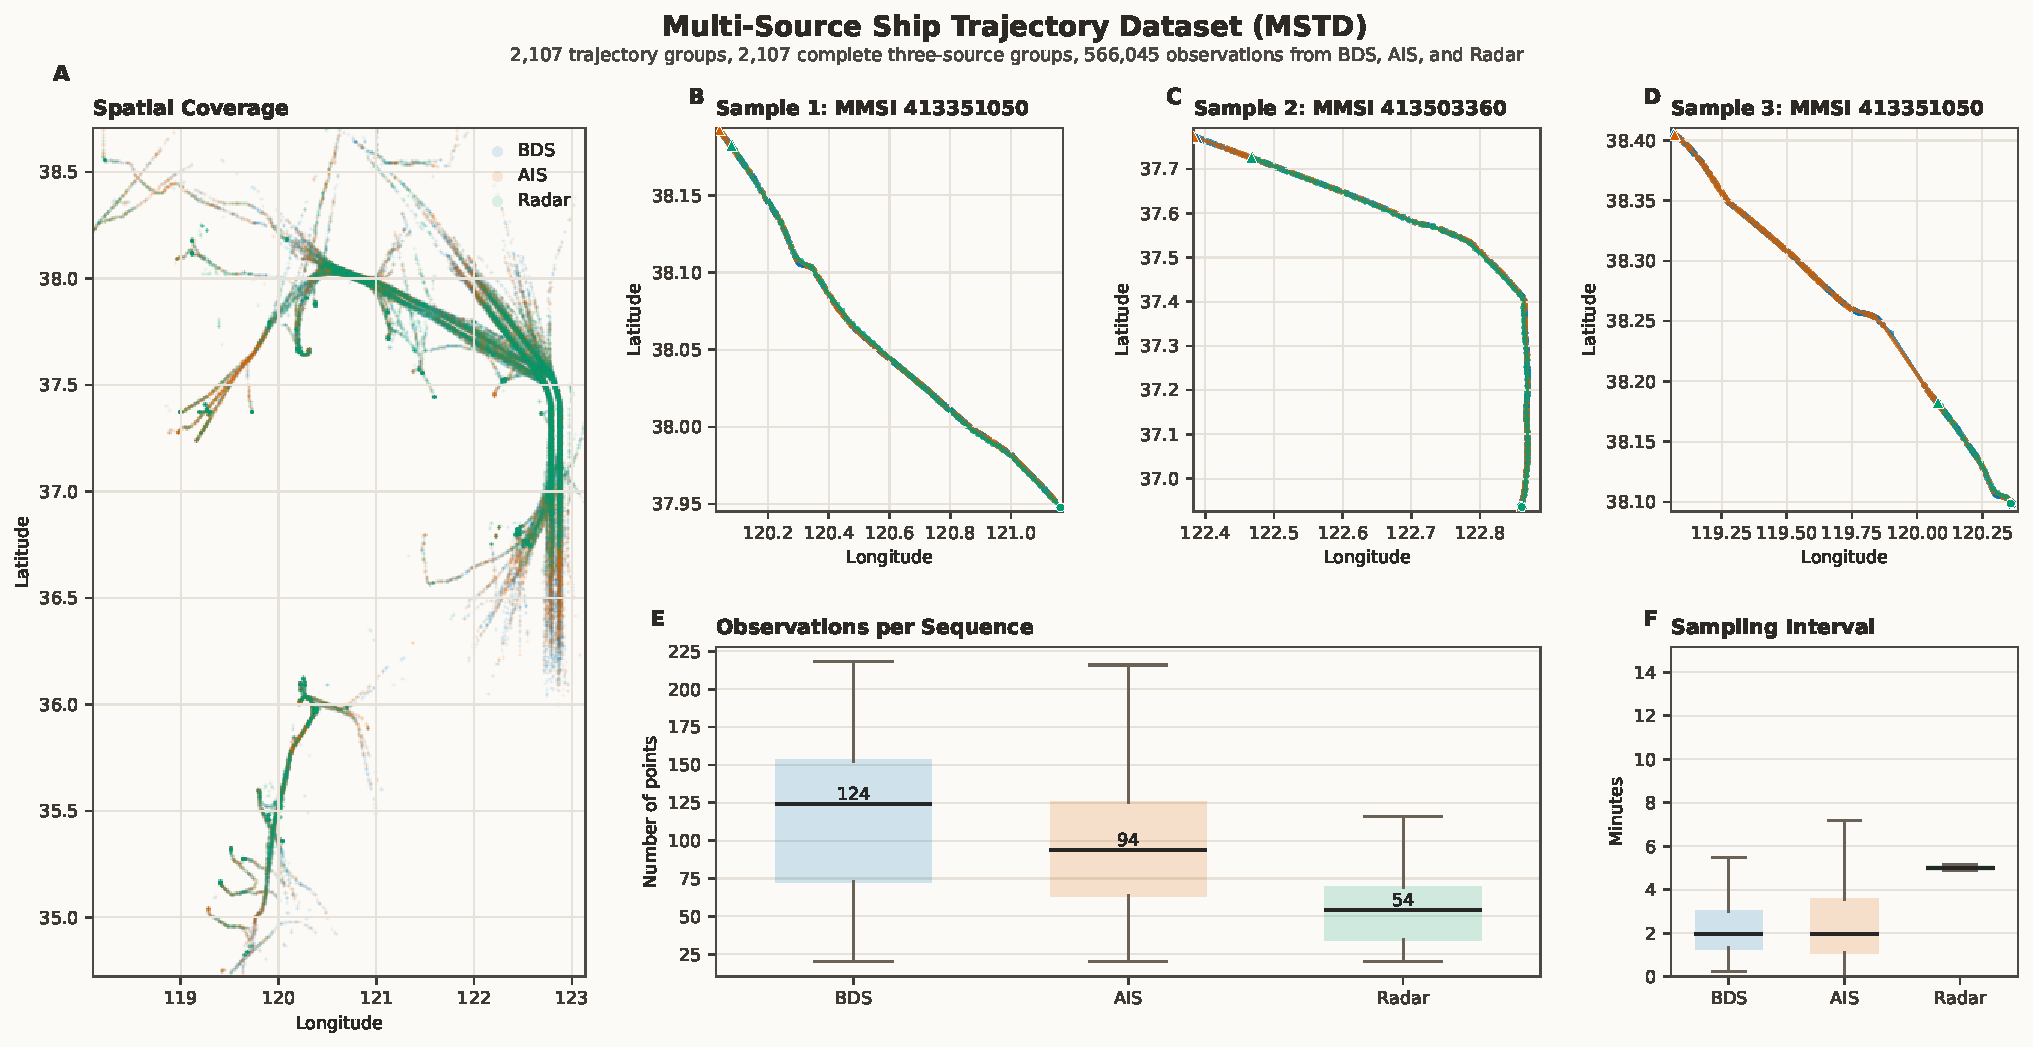
\includegraphics[width=0.99\textwidth]{figures/mstd_dataset_overview.pdf}
    \caption{Visualization of the Multi-Source Ship Trajectory Dataset (MSTD). Panel A shows the spatial coverage of BDS, AIS, and Radar observations. Panels B--D show representative associated three-source trajectory groups. Panels E and F summarize the distribution of observation counts and sampling intervals for each source. The figure highlights the weak alignment, unequal sampling density, and source-dependent continuity that motivate patch-level cross-source completion.}
    \label{fig:mstd-visualization}
\end{figure*}

For each sample, one source is selected as the target trajectory and the remaining sources are treated as optional auxiliary trajectories. This protocol supports three evaluation modes: single-source forecasting, single-auxiliary completion, and multi-auxiliary completion. Historical incompleteness is simulated using two corruption types. Empty-patch masking removes all observations inside selected historical patches, while sparse-patch masking keeps only a small number of observations in the selected patches to represent low-density monitoring regions.

All methods use the same train/validation/test split of 60\%/20\%/20\%, the same input history, the same prediction horizon, and the same normalization statistics. Hyperparameters are selected on the validation split, and the checkpoint with the lowest validation loss is evaluated on the test split. We report Test Loss, positional mean absolute error (Pos MAE), final-step mean absolute error (Final MAE), average L2 distance (Avg L2), average mean squared error (Avg MSE), and average dynamic time warping distance (Avg DTW). Lower values indicate better performance for all metrics.

\subsection{Overall Forecasting Performance}
\label{subsec:overall-performance}

The first experiment evaluates single-target forecasting without historical corruption. This setting isolates the ability of each model to encode irregular trajectory histories and predict future vessel motion before introducing auxiliary-source completion. The comparison includes classical recurrent models, patch-based time-series models, graph-based forecasting models, irregular time-series models, continuous-time models, and the proposed Traj-PathFormer. All baselines are trained and evaluated with the same no-sliding protocol so that each original trajectory group contributes only one training or testing sample.

Table~\ref{tab:overall-performance-mstd} reports the completed single-target forecasting results. Traj-PathFormer obtains the lowest Test Loss, Pos MAE, Final MAE, Avg L2, Avg MSE, and Avg DTW among the compared methods. The improvement over recurrent and continuous-time baselines indicates that time-aware patch encoding is useful for irregular maritime trajectories. The improvement over patch and graph forecasting baselines further suggests that trajectory-specific temporal queries and local patch modeling are important for ship motion extrapolation.

\begin{table*}[t]
    \centering
    \caption{Single-target no-sliding forecasting performance. Lower is better for all metrics.}
    \label{tab:overall-performance-mstd}
    \small
    \begin{tabular}{lcccccc}
        \hline
        Method & Test Loss & Pos MAE & Final MAE & Avg L2 & Avg MSE & Avg DTW \\
        \hline
        Ours & 0.0912 & 221.3403 & 396.6012 & 0.003260 & 0.00001875 & 0.032463 \\
        AGDN & 0.1672 & 322.9428 & 568.9746 & 0.004701 & 0.00003416 & 0.045685 \\
        TLSTM & 0.1533 & 304.1389 & 534.5453 & 0.004457 & 0.00003063 & 0.043179 \\
        T-PatchGNN & 0.3515 & 632.3910 & 1148.7339 & 0.009282 & 0.00008465 & 0.107036 \\
        DLinear & 0.1468 & 296.5776 & 520.4579 & 0.004362 & 0.00002915 & 0.043687 \\
        TimesNet & 0.1608 & 320.3552 & 549.0652 & 0.004652 & 0.00002963 & 0.045639 \\
        PatchTST & 0.1607 & 342.7858 & 597.5205 & 0.005077 & 0.00003174 & 0.051094 \\
        Crossformer & 0.1327 & 294.1077 & 503.8624 & 0.004281 & 0.00002766 & 0.041038 \\
        Graph WaveNet & 0.1621 & 316.8399 & 539.9712 & 0.004603 & 0.00003175 & 0.045384 \\
        MTGNN & 0.1725 & 320.6826 & 553.6057 & 0.004723 & 0.00003397 & 0.046464 \\
        StemGNN & 0.1513 & 301.2865 & 534.9033 & 0.004445 & 0.00002788 & 0.045406 \\
        CrossGNN & 0.1470 & 291.3072 & 509.4098 & 0.004220 & 0.00002559 & 0.041731 \\
        FourierGNN & 0.1424 & 304.4529 & 527.9481 & 0.004438 & 0.00002473 & 0.044792 \\
        GRU-D & 0.1505 & 299.0100 & 516.3393 & 0.004419 & 0.00002861 & 0.042718 \\
        SeFT & 0.3007 & 532.1498 & 987.2258 & 0.007802 & 0.00007024 & 0.086307 \\
        RainDrop & 0.2072 & 393.5482 & 732.4191 & 0.005834 & 0.00004123 & 0.058391 \\
        Warpformer & 0.1456 & 293.2483 & 519.3995 & 0.004280 & 0.00002633 & 0.042219 \\
        mTAND & 0.3154 & 572.5056 & 1027.1610 & 0.008375 & 0.00007512 & 0.092223 \\
        Latent-ODE & 0.1449 & 291.9276 & 505.7471 & 0.004294 & 0.00002745 & 0.041619 \\
        CRU & 0.1520 & 306.5746 & 537.9244 & 0.004482 & 0.00003031 & 0.043251 \\
        Neural Flow & 0.1305 & 274.2642 & 480.2103 & 0.004070 & 0.00002432 & 0.040065 \\
        \hline
    \end{tabular}
\end{table*}

\subsection{Robustness to Incomplete Historical Patches}
\label{subsec:missing-sparse-robustness}

The second experiment evaluates whether patch-level completion improves forecasting when historical observations are incomplete. We consider two types of incomplete history. Empty-patch corruption represents complete local sensing failure, where all observations in selected patches are removed. Sparse-patch corruption represents low-density monitoring, where only a few observations remain inside the selected patches. For each corruption level, we compare three protocols: forecasting without completion, direct source filling, and the proposed single-source cross-attention completion.

Table~\ref{tab:missing-sparse-robustness} shows that cross-attention completion consistently gives the best results across both empty and sparse patch settings. Direct source filling can reduce error when a target patch is fully empty, but it is less reliable under sparse corruption because copying auxiliary points may overwrite useful target observations or introduce source-specific offsets. In contrast, cross-attention completion transfers information at the representation level, allowing the model to use auxiliary evidence while preserving the target trajectory context.

\begin{table*}[t]
    \centering
    \caption{Robustness to empty and sparse historical patches. Lower is better for all metrics.}
    \label{tab:missing-sparse-robustness}
    \small
    \begin{tabularx}{\textwidth}{llXcccccc}
        \hline
        Corruption & Patches & Completion Protocol & Test Loss & Pos MAE & Final MAE & Avg L2 & Avg MSE & Avg DTW \\
        \hline
        Empty & 1 & None & 0.0426 & 214.0463 & 349.9421 & 0.003177 & 0.00001376 & 0.032712 \\
        Empty & 1 & Direct Source Fill & 0.0418 & 204.6442 & 332.9675 & 0.003037 & 0.00001315 & 0.031304 \\
        Empty & 1 & Single-Source Cross-Attn. & 0.0410 & 202.6891 & 330.3001 & 0.003009 & 0.00001291 & 0.031109 \\
        \hline
        Empty & 2 & None & 0.0434 & 219.3537 & 360.6593 & 0.003259 & 0.00001433 & 0.033507 \\
        Empty & 2 & Direct Source Fill & 0.0431 & 208.9927 & 340.5367 & 0.003099 & 0.00001380 & 0.031884 \\
        Empty & 2 & Single-Source Cross-Attn. & 0.0412 & 203.3165 & 331.3052 & 0.003016 & 0.00001305 & 0.031164 \\
        \hline
        Empty & 3 & None & 0.0439 & 220.9296 & 364.7376 & 0.003283 & 0.00001458 & 0.033825 \\
        Empty & 3 & Direct Source Fill & 0.0433 & 209.8891 & 341.9404 & 0.003113 & 0.00001376 & 0.032073 \\
        Empty & 3 & Single-Source Cross-Attn. & 0.0413 & 203.0973 & 331.0697 & 0.003012 & 0.00001298 & 0.031154 \\
        \hline
        Sparse & 1 & None & 0.0413 & 205.1377 & 334.2994 & 0.003044 & 0.00001301 & 0.031408 \\
        Sparse & 1 & Direct Source Fill & 0.0418 & 204.6442 & 332.9675 & 0.003037 & 0.00001315 & 0.031304 \\
        Sparse & 1 & Single-Source Cross-Attn. & 0.0409 & 202.3945 & 329.7261 & 0.003005 & 0.00001287 & 0.031072 \\
        \hline
        Sparse & 2 & None & 0.0416 & 206.4329 & 336.1953 & 0.003064 & 0.00001309 & 0.031566 \\
        Sparse & 2 & Direct Source Fill & 0.0431 & 208.9927 & 340.5367 & 0.003099 & 0.00001380 & 0.031884 \\
        Sparse & 2 & Single-Source Cross-Attn. & 0.0410 & 202.7830 & 330.3737 & 0.003010 & 0.00001297 & 0.031107 \\
        \hline
        Sparse & 3 & None & 0.0419 & 207.1303 & 337.2458 & 0.003072 & 0.00001312 & 0.031643 \\
        Sparse & 3 & Direct Source Fill & 0.0433 & 209.8891 & 341.9404 & 0.003113 & 0.00001376 & 0.032073 \\
        Sparse & 3 & Single-Source Cross-Attn. & 0.0410 & 202.5264 & 330.1328 & 0.003005 & 0.00001290 & 0.031089 \\
        \hline
    \end{tabularx}
\end{table*}

\subsection{Single-Source and Multi-Source Completion}
\label{subsec:source-completion-analysis}

The third experiment studies which auxiliary source should be used for completion. One source is selected as the target trajectory, while the other sources are used individually or jointly. The single-source setting uses one auxiliary local patch sequence. The multi-source setting uses two auxiliary local patch sequences, each with length three, and fuses them through cross-attention before reconstructing the incomplete target patch. This design evaluates whether Radar, AIS, and BDS provide complementary evidence rather than interchangeable point-wise replacements.

Table~\ref{tab:source-completion-analysis} defines the source-selection comparison for one incomplete target patch. The rows are organized by target source so that the effect of each auxiliary source can be interpreted separately. The ``None'' rows measure the cost of making predictions from incomplete target history alone. The single-source rows measure how much each auxiliary source contributes individually. The multi-source rows test whether jointly attending to two auxiliary sources provides a stronger and more stable completion signal.

\begin{table*}[t]
    \centering
    \caption{Effect of auxiliary source selection for one incomplete target patch. Lower is better for all metrics.}
    \label{tab:source-completion-analysis}
    \small
    \begin{tabularx}{\textwidth}{llXcccccc}
        \hline
        Target & Auxiliary Source(s) & Completion Protocol & Test Loss & Pos MAE & Final MAE & Avg L2 & Avg MSE & Avg DTW \\
        \hline
        AIS & None & No Completion & -- & -- & -- & -- & -- & -- \\
        AIS & BDS & Single-Source Cross-Attn. & -- & -- & -- & -- & -- & -- \\
        AIS & Radar & Single-Source Cross-Attn. & -- & -- & -- & -- & -- & -- \\
        AIS & BDS + Radar & Multi-Source Cross-Attn. & -- & -- & -- & -- & -- & -- \\
        \hline
        BDS & None & No Completion & -- & -- & -- & -- & -- & -- \\
        BDS & AIS & Single-Source Cross-Attn. & -- & -- & -- & -- & -- & -- \\
        BDS & Radar & Single-Source Cross-Attn. & -- & -- & -- & -- & -- & -- \\
        BDS & AIS + Radar & Multi-Source Cross-Attn. & -- & -- & -- & -- & -- & -- \\
        \hline
        Radar & None & No Completion & -- & -- & -- & -- & -- & -- \\
        Radar & AIS & Single-Source Cross-Attn. & -- & -- & -- & -- & -- & -- \\
        Radar & BDS & Single-Source Cross-Attn. & -- & -- & -- & -- & -- & -- \\
        Radar & AIS + BDS & Multi-Source Cross-Attn. & -- & -- & -- & -- & -- & -- \\
        \hline
    \end{tabularx}
\end{table*}

\subsection{Local Auxiliary Patch Length}
\label{subsec:local-patch-length-ablation}

The fourth experiment verifies the choice of using three auxiliary patches for local cross-attention completion. A very short auxiliary context may not contain enough motion evidence when the target patch is missing or sparse. Conversely, a long auxiliary context may introduce temporally distant observations that are weakly related to the missing target region. We therefore compare interpolation, direct source filling, and cross-attention completion with one to eight auxiliary patches.

Table~\ref{tab:local-patch-length-ablation} is structured to identify the best local auxiliary window. The interpolation and direct-filling rows are non-attention baselines, while the cross-attention rows test how the model behaves as the auxiliary context grows. The expected operating point is the smallest window that provides stable gains without adding distant-source noise or unnecessary computation.

\begin{table*}[t]
    \centering
    \caption{Ablation on the number of auxiliary patches used for completion. Lower is better for all metrics.}
    \label{tab:local-patch-length-ablation}
    \small
    \begin{tabularx}{\textwidth}{lXcccccc}
        \hline
        Strategy & Auxiliary Context & Test Loss & Pos MAE & Final MAE & Avg L2 & Avg MSE & Avg DTW \\
        \hline
        Linear Interpolation & Target source only & -- & -- & -- & -- & -- & -- \\
        Direct Source Fill & One auxiliary source & -- & -- & -- & -- & -- & -- \\
        Cross-Attn. & 1 auxiliary patch & -- & -- & -- & -- & -- & -- \\
        Cross-Attn. & 2 auxiliary patches & -- & -- & -- & -- & -- & -- \\
        Cross-Attn. & 3 auxiliary patches & -- & -- & -- & -- & -- & -- \\
        Cross-Attn. & 4 auxiliary patches & -- & -- & -- & -- & -- & -- \\
        Cross-Attn. & 5 auxiliary patches & -- & -- & -- & -- & -- & -- \\
        Cross-Attn. & 6 auxiliary patches & -- & -- & -- & -- & -- & -- \\
        Cross-Attn. & 7 auxiliary patches & -- & -- & -- & -- & -- & -- \\
        Cross-Attn. & 8 auxiliary patches & -- & -- & -- & -- & -- & -- \\
        \hline
    \end{tabularx}
\end{table*}

\subsection{Model Ablation}
\label{subsec:ablation-study}

The final experiment evaluates the contribution of the main architectural components. Each variant removes or replaces one design while keeping the dataset split, corruption protocol, training schedule, and evaluation metrics fixed. This controlled setting separates the effect of time-aware encoding, future-step querying, completion, multi-source fusion, temporal patch bias, and intra-patch modeling.

Table~\ref{tab:model-ablation} lists the planned ablation variants. The full model corresponds to Traj-PathFormer with time-aware patch embedding, temporal patch attention, local cross-attention completion, and the time-conditioned future query decoder. The ablated variants are chosen to answer whether each component is necessary, whether direct source filling can replace learned completion, and whether multi-source fusion provides benefits beyond a single auxiliary trajectory.

\begin{table*}[t]
    \centering
    \caption{Model ablation on MSTD. Lower is better for all metrics.}
    \label{tab:model-ablation}
    \small
    \begin{tabularx}{\textwidth}{lXcccccc}
        \hline
        Variant & Description & Test Loss & Pos MAE & Final MAE & Avg L2 & Avg MSE & Avg DTW \\
        \hline
        Full Model & Complete Traj-PathFormer & -- & -- & -- & -- & -- & -- \\
        w/o Time-Aware Encoding & Remove temporal interval encoding from patch and future queries & -- & -- & -- & -- & -- & -- \\
        w/o Future Query Decoder & Replace time-conditioned future queries with a global prediction head & -- & -- & -- & -- & -- & -- \\
        w/o Completion Branch & Predict from incomplete history without patch completion & -- & -- & -- & -- & -- & -- \\
        Direct Source Fill & Replace cross-attention completion with direct auxiliary-source filling & -- & -- & -- & -- & -- & -- \\
        Single-Source Completion Only & Disable multi-source auxiliary fusion & -- & -- & -- & -- & -- & -- \\
        w/o Temporal Patch Bias & Replace temporally biased patch attention with standard self-attention & -- & -- & -- & -- & -- & -- \\
        w/o Intra-Patch Attention & Replace point-level intra-patch attention with masked mean pooling & -- & -- & -- & -- & -- & -- \\
        \hline
    \end{tabularx}
\end{table*}

% To print the credit authorship contribution details
\printcredits
%% Loading bibliography style file
%\bibliographystyle{model1-num-names}
\bibliographystyle{cas-model2-names}

% Loading bibliography database
\bibliography{cas-refs}


%\vskip3pt

\end{document}
